% Copyright (c)  2005-2010 EDF-EADS-PHIMECA.
% Permission is granted to copy, distribute and/or modify this document
% under the terms of the GNU Free Documentation License, Version 1.2
% or any later version published by the Free Software Foundation;
% with no Invariant Sections, no Front-Cover Texts, and no Back-Cover
% Texts.  A copy of the license is included in the section entitled "GNU
% Free Documentation License".
\renewcommand{\filename}{docUC_StocProc_SpectralModel_Estimation.tex}
\renewcommand{\filetitle}{UC : Estimation of a spectral model}

% \HeaderNNIILevel
% \HeaderIILevel
\HeaderIIILevel

\index{Stochastic Process!Spectral Model}


Let $\vect{X}(\omega,t)$ be a stationary process with zero mean and unilateral spectral density function defined in (\ref{univG}).\\

This objective of this use case is to estimate a spectral density function $f$ from data. The challenges may differ depending on \emph{observations} :

\begin{itemize}
 \item if the observations correspond to  several independent  realizations of a  process (stored in a $ProcessSample$ object), a \emph{statistical estimate} is performed using statistical average of a realization-based estimator;
 \item if the observations correspond to the realization of a  process  at different instants (stored in a  $TimeSeries$ object), the process being observed during a long period of time, an\emph{ergodic estimate} is performed using a time average of an ergodic-based estimator.
\end{itemize}
 
We can also distinguish $two$ families of estimation methods : parametric methods where the underlying stationary stochastic process $\vect{X}(\omega,t)$ has a specified structure which parameters have to be estimated, and  non parametric methods where the estimation of the spectrum is done without any particular hypothesis of structure.\\

The \emph{non parametric} $Welch$ method is used for estimating the spectral density at different frequencies. This method is known to be performant. Let us introduce the main steps of the algorithm on a time series. \\ 
Let $\vect{X}(j), \ j = 0, 1,...,N-1$ a time series defined from a stationary second order stochastic process with $\mathbb{E}(\vect{X}) = 0$, with the time grid $[0, T]$.
With the stationary hypothesis, we assume that $\vect{X}$ have a spectral density $f(\omega)$ with $| \omega | \leq \frac{T}{2}$. 
The method is based on the segmentation of the time series into $K$ segments of length $L$, possibly overlapping (size of overlap $R$).\\
Let $\vect{X}_{1}(j), \ j = 0, 1,...,L-1$ be the first such segment. Then :
\begin{equation*}
\vect{X}_{1}(j) = \vect{X}(j) , \ j = 0, 1,...,L-1
\end{equation*}
Applying the same decomposition, 
\begin{equation*}
 \vect{X}_{2}(j) = \vect{X}(j + (L - R)) , \ j = 0, 1,...,L-1
\end{equation*}
and finally :
\begin{equation*}
 \vect{X}_{K}(j) = \vect{X}(j + (K-1)(L-R)) , \ j = 0, 1,...,L-1
\end{equation*}

The objective is to get a statistical estimator from these $K$ segments. We define the \emph{periodogram} associated with the segment $\vect{X}_k$ by:
\begin{eqnarray*}
  \vect{X}_{k}(f_p,T)&=&\Delta t\sum_{n=0}^{L-1}\vect{x}(n\Delta t)\exp\left[\frac{-j2\pi pn}{N}\right], \quad p=0,\dots, L-1\\
  \hat{G}_{\vect{x}}(f_p,T)&=&\frac{2}{T}\vect{X}_{k}(f_p,T)\,{\vect{X}_{k}(f_p,T)^*}^t,\quad p=0,\dots,L/2-1
\end{eqnarray*}
with $\Delta t=\frac{T}{N}$ and $f_p=\frac{p}{T}=\frac{p}{N}\frac{1}{\Delta t}$.\\

It has been proven that the \emph{periodogram} has bad statistical properties. Indeed, two quantities summarize the properties of an estimator: 
its \emph{bias} and its \emph{variance}. 
The bias is the expected error one makes on the average using only a finite number of time series of finite length, whereas the covariance is the expected fluctuations of 
the estimator around its mean value. For the periodogram, we have:

\begin{itemize}
\item Bias$=\mathbb{E}[\hat{G}_{\vect{x}}(f_p, T)-G_{\vect{X}}(f_p)]=(\frac{1}{T}W_B(f_p, T)-\delta_0)*G_{\vect{X}}(f_p)$ where $W_B(f_p, T) = \left(\frac{\sin\pi fT}{\pi fT}\right)^2$ is the squared module of the Fourier transform of the function $w_B(t, T)$ (\emph{Barlett window}) defined by:
  \begin{equation}
    w_B(t, T) = \mathbf{1}_{[0,T]}(t)
  \end{equation}
 This estimator is \emph{biased} but this bias vanishes when $T\rightarrow\infty$ as $\lim_{T\rightarrow\infty} \frac{1}{T}W_B(f_p, T)=\delta_0$.
\item Covariance$=\frac{1}{T}W_B(f_p, T)*G_{\vect{X}}(f_p)\rightarrow G_{\vect{X}}(f_p)$ as $T\rightarrow\infty$, 
which means that the fluctuations of the periodogram are of the same order of magnitude as the quantity to be estimated and thus the estimator is not convergent. 
\end{itemize}

The periodogram's lack of convergence may be easily fixed if we  consider the \emph{averaged periodogram} over $K$ independent time series or segments:
\begin{equation}
  \hat{G}_{\vect{x}}(f_p,T)=\frac{2}{KT}\sum_{k=0}^{K-1}\vect{X}^{(k)}(f_p,T)\vect{X}^{(k)}(f_p,T)^t
\end{equation}

The averaging process has no effect on the significant bias of the periodogram.
 
The use of a \emph{tapering window} $w(t, T)$ may significantly reduce it. The time series $\vect{x}(t)$ is replaced by a tapered time series $w(t, T)\vect{x}(t)$ in the 
computation of $\vect{X}(f_p,T)$. One gets :
\begin{equation}
  \mathbb{E}[\hat{G}_{\vect{x}}(f_p, T)-G_{\vect{X}}(f_p)=(\frac{1}{T}W(f_p, T)-\delta_0)*G_{\vect{X}}(f_p)
\end{equation}
where $W(f_p, T)$ is the square module of the Fourier transform of $w(t, T)$ at the frequency $f_p$. 
A judicious choice of tapering function such as the \emph{Hanning window} $w_H$ can dramatically reduce the bias of the estimate:
\begin{equation}\label{HamEff}
  w_H(t, T) = \sqrt{\frac{8}{3}}\left(1-\cos^2\left(\frac{\pi t}{T}\right)\right)\mathbf{1}_{[0,T]}(t)
\end{equation}

OpenTURNS builds an estimation of the spectrum on a $TimeSeries$ by fixing the number of segments, the $overlap$ size parameter and a $FilteringWindows$. The available ones are : 
\begin{itemize}
 \item The $Hamming$ window
\begin{equation}
  w(t, T) = \sqrt{\frac{1}{K}}\left(0.54-0.46\cos^2\left(\frac{2 \pi t}{T}\right)\right)\mathbf{1}_{[0,T]}(t)
\end{equation}
with $K$ = $\sqrt{0.54^2 + \frac{1}{2} 0.46^2}$
 \item The $Hanning$ window described in (\ref{HamEff}) which is supposed to be the most usefull.
\end{itemize}
The result consists in a $UserDefinedSpectralModel$ which is simple to manipulate. \\

Furthermore, OpenTURNS build an estimation of the spectral function on a process sample  by considering that $k-th$ segment is the $k-th$ time series  of the process sample .\\

Details on each object may be found in the User Manual  (\href{OpenTURNS_UserManual_TUI.pdf}{see User Manual - StochasticProcess}).\\


\requirements{

  \begin{description}
  \item[$\bullet$] number of segments {\itshape mySegmentNumber}
  \item[type:]  integer
  \end{description}

  \begin{description}
  \item[$\bullet$] size of overlap {\itshape myOverlapSize}
  \item[type:]  integer
  \end{description}

  \begin{description}
  \item[$\bullet$] a time series {\itshape myTimeSeries}
  \item[type:]  TimeSeries
  \end{description}

  \begin{description}
  \item[$\bullet$] a set of time series {\itshape mySample}
  \item[type:]  ProcessSample
  \end{description}

}
{

  \begin{description}
  \item[$\bullet$] a spectral model : {\itshape myEstimatedModel}
  \item[type:]  UserDefinedSpectralModel
  \end{description}

}

\textspace\\
Python script for this Use Case :

\begin{lstlisting}

 # Build a factory 
 myFactory = WelchFactory(Hanning(), mySegmentNumber , myOverlapSize)

 # Estimation on a TimeSeries
 myEstimateModel = myFactory.build(myTimeSeries)

 # Change the filtering window 
 myFactory.setFilteringWindows(Hamming())

 # Get the FFT algorithm
 myFFT = myFactory.getFFTAlgorithm()

 # Get the frequencyGrid - Return result is a RegularGrid
 frequencyGrid = myEstimateModel.getFrequencyGrid()
    
 # Estimation on a ProcessSample
 myEstimateModel = myFactory.build(mySample)

\end{lstlisting}

\textspace\\
The example illustrated below makes an estimation on a sample issued from a $SpectralNormalProcess$ with parameters :
\begin{itemize}
 \item  timeGrid ($RegularGrid$) = $[0, 102.3]$ with $step=0. 1$
 \item  $SpectralModel$ is the Cauchy model with $\vect{\lambda}=(5)$, $\vect{a}=(3)$ 
 \item Size of sample is $1000$
\end{itemize}

Figures (\ref{welch_validation}) draws the graphs of the spectrum's norm for the computed frequencies. 
The result is compared with the initial model.
We makes an estimation of the spectral density $f$ and we compare this last one to the true Cauchy model. 


\begin{figure}[H]
\begin{center}
  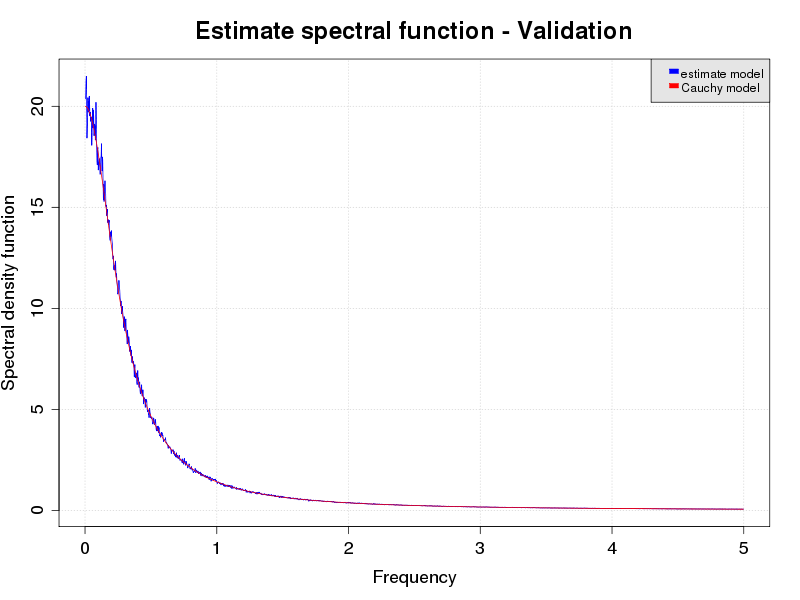
\includegraphics[width=7cm]{welchValidation.png}
  \caption{Welch comparison }
  \label{welch_validation}
\end{center}
\end{figure}



